% Chapter 2

\chapter{Conception et Développement} % Chapter title

\label{ch:2} % For referencing the chapter elsewhere, use \autoref{ch:3} 

De prime abord, il est important de souligner que la création d'un \ac{llm} est un processus coûteux et exigeant en termes de données. Les modèles de langage existants, tels que GPT-4 \cite{openai2023gpt4}, ont été développés avec une quantité massive de données et une puissance de calcul considérable. Cependant, pour adapter ces modèles au contexte juridique congolais, il serait peu pratique, voire impossible, de construire un \ac{llm} à partir de zéro en raison de contraintes de ressources.

Inspiré par Heydar Soudani \cite{soudani2024fine}, notre approche consiste à utiliser un modèle de langage existant comme point de départ (voir Table~\ref{table:llm-models}). En prenant un modèle pré-entraîné, nous pouvons bénéficier des connaissances et des capacités linguistiques déjà intégrées dans le modèle. Nous chercherons ensuite à affiner ce modèle pré-entraîné pour le rendre spécifique au système juridique congolais. Pour ce faire, nous utiliserons deux méthodes principales : le \ac{ft} et le \ac{rag}.

\paragraph{\acf{ft}} \hspace{0pt}

Le \ac{ft} implique de prendre un modèle de langage pré-entraîné, tel que GPT-4, et de le spécialiser pour le domaine spécifique du système juridique Congolais. Cette méthode consiste à ajuster les poids du modèle en le nourrissant avec des données spécifiques au contexte juridique Congolais. En utilisant des corpus de textes juridiques, des décisions de justice et d'autres ressources pertinentes, nous entraînerons le modèle à comprendre et à générer des réponses cohérentes et précises aux questions juridiques \cite{yue2023disclawllm}.

\paragraph{\acf{rag}} \hspace{0pt}

En parallèle, nous utiliserons également l'approche du \ac{rag}, qui combine la génération de texte avec des techniques de recherche d'informations. Le \ac{rag} permet au chatbot d'accéder à une base de connaissances juridiques étendue et de récupérer des informations pertinentes en réponse aux requêtes des utilisateurs. En utilisant des index de recherche efficaces et des algorithmes de récupération d'informations, le chatbot peut fournir des réponses bien informées en s'appuyant sur une grande variété de sources \cite{lewis2021retrievalaugmented}.

En définitive, La conception et le développement présentés dans ce mémoire s'articulent autour de deux axes principaux. D'une part, nous nous concentrerons sur le modèle \ac{llm}, en suivant toutes les étapes de conception et de développement détaillées dans la section \ref{ch:1:section:ml-process}. Ce processus englobe la collecte initiale des données brutes jusqu'au déploiement final du modèle sélectionné dans un environnement de production. D'autre part, l'attention sera également portée sur le développement du chatbot, qui agit en tant qu'application web. Cette interface utilisateur servira de pont pour accéder au modèle \ac{llm}, facilitant ainsi l'interaction entre les utilisateurs et le système juridique Congolais à travers le chatbot. 

Ce dernier ne représente pas seulement un outil d'accès, mais aussi une manière intuitive et efficace de mettre en application les capacités du modèle \ac{llm}, permettant aux utilisateurs d'obtenir des réponses et des informations juridiques pertinentes de manière interactive.

\section{Les données}

Compte tenu de nos contraintes et objectifs (voir Section~\ref{ch:0:section:limitaions}), les données n'ont pas besoin d'être structurées selon un format particulier, à condition qu'elles soient disponibles sous forme textuelle. Cette flexibilité permet d'exploiter une large variété de sources d'information juridique sans nécessiter de processus de prétraitement complexe pour adapter les données à un format spécifique.

Notre jeu de données sera principalement constitué de documents juridiques provenant de diverses sources officielles et spécialisées, afin d'englober une vaste étendue de la législation et de la doctrine juridique congolaise.

Il est à noter que, bien que les données ne requièrent pas un format spécifique, leur qualité textuelle est essentielle. Cela implique un travail de vérification pour s'assurer de la fiabilité, de la pertinence et de l'actualité des informations collectées. Ce processus permettra de minimiser les erreurs et les ambiguïtés dans les réponses fournies par le chatbot, assurant ainsi une assistance juridique de qualité aux utilisateurs.

\subsection{Les sources d'informations}

\begin{table}[h]
\centering
\begin{tabular}{|l|p{10cm}|}
    \hline
    \textbf{Source} & \textbf{Description} \\
    \hline
    Journal Officiel & Publications officielles qui contiennent les nouvelles lois, décrets, et annonces légales, offrant une source à jour des évolutions législatives. \\
    \hline
    Lois et Décrets & Textes législatifs et réglementaires qui forment la base du système juridique congolais, essentiels pour comprendre le cadre légal en vigueur. \\
    \hline
    Jurisprudences & Décisions de justice issues des tribunaux, fournissant des exemples concrets d’application des lois et des interprétations juridiques. \\
    \hline
    Articles d’Actualité Juridique & Articles publiés par des spécialistes et des médias juridiques, offrant des analyses et des commentaires sur les évolutions récentes du droit et les cas d’intérêt. \\
    \hline
    Doctrine & Contributions d’experts dans le domaine juridique, y compris des analyses détaillées, des critiques, et des interprétations de divers aspects du droit. \\
    \hline
\end{tabular}
\caption{Sources d'information dans le système juridique Congolais}
\label{table:sources-legales-congo}
\end{table}

La numérisation et l'adoption croissante d'Internet en République Démocratique du Congo (RDC) ont considérablement facilité l'accès aux documents légaux officiels. Désormais, un nombre croissant de ces documents est accessible librement en ligne, offrant une opportunité sans précédent pour la recherche et l'analyse juridique. Des plateformes telles que Leganet.cd \footnote{\href{https://leganet.cd}{https://leganet.cd}} jouent un rôle crucial dans l'agrégation et la diffusion de ces documents, constituant ainsi une ressource inestimable pour les praticiens du droit, les chercheurs, et le grand public intéressé par le droit congolais.

Dans ce cadre nous envisageons d'explorer ces diverses sources en ligne. L'objectif est de collecter un large éventail de documents afin de capturer l'étendue et la profondeur du cadre juridique congolais. Cette démarche vise non seulement à fournir à notre modèle une richesse de connaissances et de perspectives sur le droit congolais mais aussi à garantir que les réponses générées soient à la fois informées et pertinentes, reflétant fidèlement les principes et les pratiques juridiques actuels.

Pour faciliter la découverte et l'exploration de ces ressources en ligne, nous envisageons d'utiliser l'\acs{api} Google Custom Search \footnote{\href{https://developers.google.com/custom-search/v1/introduction}{https://developers.google.com/custom-search/v1/introduction}}. Cet outil nous permettra d'automatiser la recherche et de visualiser rapidement les résultats, identifiant ainsi les sites les plus pertinents et fiables où les documents juridiques Congolais sont disponibles. Cette approche automatisée nous aidera à optimiser le processus de collecte de données, en assurant une couverture des sources d'information juridique pertinentes pour notre modèle.

\newpage
\paragraph{Les mots clés} \hspace{0pt}

Les mots-clés jouent un rôle crucial dans le processus de recherche, particulièrement lorsqu'il s'agit de collecter des données spécifiques à un domaine tel que le Droit Congolais. Ils servent de fondement pour affiner les requêtes de recherche et accéder efficacement à l'information pertinente.

\begin{listing}[!ht]
\begin{minted}{python}
keywords = [
    "Constitution", "civil", "Code pénal",
    "Code de travail", "Code foncier ", "Jurisprudence",
    "Droits humains", "Justice transitionnelle", "Droit minier",
    "l'environnement", "commercial", "sociétés",
    "Propriété intellectuelle", "famille", "Violence sexuelle et droit",
    "international humanitaire", "Institutions judiciaires congolaises", 
    "Réforme judiciaire",
    "Lutte contre la corruption", "affaires", "Arbitrage et médiation",
    "bancaire et financier congolais", "fiscal congolais", 
    "Contrats et obligations en congolais",
    "assurances", "santé", "l'éducation",
    "technologies de l'information", "humanitaire",
    "Participation politique et droit"
]
\end{minted}
\caption{Liste des mots clés à utiliser pour la recherche.}
\label{appendix:code:python:search-keywords}
\end{listing}

Cette liste englobe une gamme étendue de domaines juridiques, allant du cadre constitutionnel et législatif général à des domaines plus spécifiques tels que le droit minier, le droit fiscal, et le droit des affaires. Elle inclut également des aspects liés à la jurisprudence, aux publications officielles, et aux analyses d'experts.

Après avoir établi notre liste de mots-clés, nous pouvons créer une fonction qui interagit avec l'\ac{api} Google Custom Search. Cette fonction se sert de la bibliothèque \textbf{Requests} \footnote{\href{https://pypi.org/project/requests/}{https://pypi.org/project/requests/}} pour lancer une requête GET vers l'\acs{url} de l'\acs{api}, en incorporant les paramètres que nous avons spécifiés. Les données renvoyées par l'\acs{api} nous parviennent sous forme de \ac{json}.

\begin{listing}[!ht]
\begin{minted}{python}
params = {
  'q': query,
  'orTerms': ' '.join(keywords).lower(),
  'start': start,
  'key': "xxxxxxxxxxxxxxxxxxxxxxxxxxxxxxxx",
  'cx': 'xxxxxxxxxxxxxxxxxxxx',
  'lr': 'lang_fr',
  'fileType': 'pdf',
  'num': 10
}
\end{minted}
\caption{Dictionnaire des paramètres utile à l'utilisation de l'\acs{api} Google Custom Search}
\label{appendix:code:python:search-google-params}
\end{listing}

Le dictionnaire \textbf{params} contient plusieurs paramètres configurés pour la requête de recherche, des explications détaillées sur l'utilisation des paramètres sont disponible sur la documentation \footnote{\href{https://developers.google.com/custom-search/v1/reference/rest/v1/cse/list}{https://developers.google.com/custom-search/v1/reference/rest/v1/cse/list}} :

\textbf{q}: Le terme principal de la recherche. \\
\textbf{orTerms}: Une chaîne de caractères contenant tous les mots-clés joints par un espace, servant à élargir la recherche à ces termes connexes. \\
\textbf{fileType}: Restreint les résultats aux fichiers d'un type spécifique, ici des \acs{pdf}. \\
\textbf{lr} : Limite la recherche aux documents dans la langue spécifiée, ici le français. \\
\textbf{num}: Détermine le nombre de résultats de recherche à retourner, ici 10 résultats.

La fonction est conçue pour récupérer les résultats d'une seule page à la fois. Pour explorer un ensemble plus large de résultats, nous allons nous appuyer sur la constante \textbf{MAX PAGES}. En procédant à une itération, nous collecterons les résultats de plusieurs pages jusqu'à atteindre la limite fixée par \textbf{MAX PAGES}.

\paragraph{Agrégation des sources} \hspace{0pt}

\begin{listing}[!ht]
\begin{minted}{python}
import requests
import json
import pickle

MAX_PAGES = 10

def search(start=1):
    url = 'https://www.googleapis.com/customsearch/v1'
    query = 'droit congolais'
    response = requests.get(url, params=params)
    return response.json()

try:
    websites = []
    for page in range(1, MAX_PAGES + 1):
        next_page = ((page - 1) * 10) + 1
        results = search(next_page)
        websites.extend(results.get("items", []))

    with open('data.pickle', 'wb') as f:
        pickle.dump(websites, f)
except Exception as e:
    raise e
\end{minted}
\caption{Fonction de recherche via l'\acs{api} Google Custom Search}
\label{appendix:code:python:search-google-function}
\end{listing}

Après avoir recueilli les résultats, nous exploitons la bibliothèque \textbf{Pandas} \footnote{\href{https://pandas.pydata.org/}{https://pandas.pydata.org/}}, qui facilite à la fois la visualisation des données et leur enregistrement dans un fichier au format \ac{csv}.

\begin{listing}[!ht]
\begin{minted}{python}
import pandas as pd 

rows = []
for item in websites:
    row = {
        'Title': item.get('title'),
        'Link': item.get('link'),
        'Snippet': item.get('snippet')
    }
    rows.append(row)

df = pd.DataFrame(rows)
df.head(100)
\end{minted}
\caption{Visualisation et exportation avec Pandas}
\label{appendix:code:python:search-google-visualization}
\end{listing}


\begin{figure}[H]
    \centering
    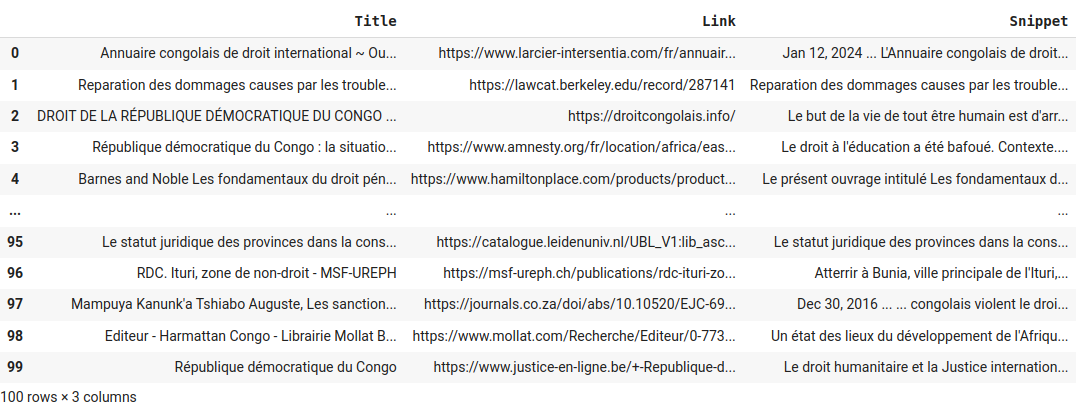
\includegraphics[width=15cm]{gfx/fig-google-search-result.png}
    \caption{Résultat de la recherche via L'\acs{api} Google Custom Search}
    \label{fig:google-search-result}
\end{figure}

Suite à l'emploi de l'\acs{api}, nous avons réussi à récolter plus de 100 résultats distincts, couvrant une variété de sites et de plate-formes dédiés au domaine juridique, et plus spécifiquement au contexte Congolais. Ces résultats nous ouvre la voie vers l'étape suivante de notre processus de collecte de données.

\subsection{Collecte des données}

La collecte de données peut être effectuée via diverses méthodes, dépendant de la nature des données visées et du contexte d'utilisation. Parmi les techniques les plus courantes, on trouve les enquêtes et sondages, l'analyse documentaire, l'observation, et l'exploration de données en ligne. Chacune de ces méthodes a ses propres avantages et inconvénients en termes de coût, de temps, de précision et de couverture des données.

Dans le cadre de notre projet, nous avons opté pour le web scraping comme technique principale de collecte de données. Le web scraping est une méthode d'extraction automatique de données à partir de sites web. Cette technique nous permet de récupérer efficacement un grand volume de documents, en particulier des fichiers \acs{pdf} liés au droit congolais, disponibles sur divers sites et plateformes spécialisés.

Le web scraping repose sur l'utilisation de scripts ou de programmes qui envoient des requêtes aux serveurs web, analysent le \acs{html} de la page pour identifier et extraire les informations nécessaires, et sauvegardent ces informations dans un format structuré pour une utilisation ultérieure. Dans notre cas, cette méthode est particulièrement pertinente pour télécharger automatiquement une multitude de documents juridiques, ce qui constitue une ressource inestimable pour notre base de données \cite{Chakrabarti_2002}.
 
\subsubsection{Conception d'un web crawler}

Un web crawler, également connu sous le nom de web scraper ou spider, est un logiciel conçu pour parcourir automatiquement le \ac{www} en suivant les liens entre les pages web. Il est principalement utilisé pour indexer le contenu des sites web, permettant aux moteurs de recherche de collecter, classer et servir les informations recherchées par les utilisateurs. Le processus implique la visite d'une page web, la lecture de son contenu, l'extraction des liens, puis le suivi de ces liens vers d'autres pages, et ainsi de suite, formant une toile étendue de données recueillies \cite{frwiki:205243717, Chakrabarti_2002, BRIN1998107}.

Le fonctionnement d'un web crawler, tel qu'initialement conceptualisé par Larry Page, repose sur un principe fondamental relativement simple, mais puissant dans sa capacité à organiser l'information sur le web. En substance, le processus peut être décrit par quelques étapes de base codées : le crawler commence par visiter une page web spécifiée, extrait tous les liens présents sur cette page, les enregistre pour un suivi ultérieur, puis répète ce processus de manière récursive pour chaque nouveau lien découvert. Ce mécanisme permet au crawler de naviguer à travers le vaste réseau du web, en cataloguant les ressources trouvées chemin faisant.

\subsubsection{Notre approche}

Dans notre cas, l'objectif s'affine vers une recherche plus ciblée : nous visons spécifiquement à localiser et récupérer des documents au format \ac{pdf}. Ce choix implique une adaptation du processus de crawl standard pour filtrer les liens et ne retenir que ceux qui mènent directement à des fichiers \ac{pdf}. En d'autres termes, notre crawler est conçu pour non seulement suivre les liens, mais aussi pour identifier et sauvegarder les chemins vers des documents \ac{pdf}, en ignorant les autres types de fichiers ou de contenu web. Cette spécialisation permet une collecte de données plus efficace et pertinente pour nos besoins de recherche juridique, garantissant que seuls les documents correspondant à nos critères soient téléchargés et stockés pour une analyse ultérieure.

\begin{figure}[H]
    \centering
    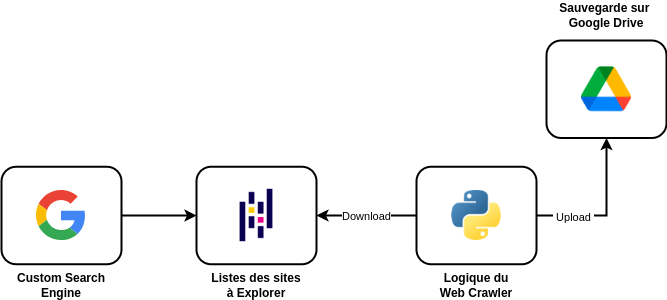
\includegraphics[width=15cm]{gfx/fig-crawler-architecture.png}
    \caption{Architecture du web crawler [le nôtre]}
    \label{fig:crawler-architecture}
\end{figure}

Comme illustré dans la figure~\ref{fig:crawler-architecture}, notre méthodologie s'aligne étroitement sur le modèle éprouvé par l'architecture de Google \cite{BRIN1998107}. Le point d'entrée de notre processus est l'utilisation de l'API Google Custom Search pour générer un inventaire de sites web spécialisés dans le droit congolais. Cette première récolte de données est ensuite convertie en un DataFrame \footnote{\href{https://pandas.pydata.org/docs/reference/api/pandas.DataFrame.html}{https://pandas.pydata.org/docs/reference/api/pandas.DataFrame.html}} Pandas, ce qui facilite la visualisation et le filtrage des données pour affiner notre recherche. Après avoir épuré cette liste, un script Python prend le relais, parcourant méthodiquement les sites pour y télécharger les fichiers \ac{pdf} disponibles. Enfin, dans la dernière étape de notre flux de travail, les \ac{pdf} ainsi collectés sont stockés sur Google Drive \footnote{\href{https://developers.google.com/drive/api/guides/about-sdk}{https://developers.google.com/drive/api/guides/about-sdk}}, assurant leur sauvegarde dans le cloud et permettant un accès aisé pour des analyses futures.

\paragraph{Implémentation itérative} \hspace{0pt}

\begin{listing}[!ht]
\begin{minted}{python}
import requests
from bs4 import BeautifulSoup

def crawl_link(url, from_root = False):
    response = requests.get(url)
    soup = BeautifulSoup(response.content, 'html.parser')
    links = soup.find_all('a', href=True)

    for link in links:
        href = link.get('href')
        if from_root:
            base = urlparse(url)
            href = f'{url}{href}'
        if href and href.endswith('.pdf'):
            download_pdf(href, DOWNLOAD_PATH)
            print(f'Downloaded {href}')
\end{minted}
\caption{Implémention itérative du crawler}
\label{appendix:code:python:iterative-crawl-function}
\end{listing}

Le script (implémentation itérative) principal de notre crawler est bâti sur l'usage de deux puissantes bibliothèques Python : requests et BeautifulSoup \footnote{\href{https://pypi.org/project/beautifulsoup4/}{https://pypi.org/project/beautifulsoup4/}}. requests  est la porte d'entrée pour accéder aux contenus des sites web en récupérant leur code \ac{html}.

Une fois le contenu \ac{html} obtenu, c'est là qu'intervient \textbf{BeautifulSoup}, une bibliothèque qui se distingue par sa capacité à analyser et à extraire des informations à partir de documents \ac{html} et \ac{xml}. Grâce à BeautifulSoup, nous pouvons naviguer dans la structure de la page web, parcourir les différents éléments du \ac{dom}, et extraire précisément les données qui nous intéressent. Elle offre une variété de méthodes pour filtrer les éléments de la page, tels que les liens, en fonction de leur balisage et de leurs attributs \cite{frwiki:203869267}.

Dans la pratique, notre script exploite BeautifulSoup pour identifier spécifiquement les liens de téléchargement de fichiers \ac{pdf}. Nous pouvons isoler ces éléments grâce à leurs attributs distinctifs (par exemple, href se terminant par .pdf) et récupérer les \acs{url}s nécessaires pour lancer le téléchargement.

\paragraph{Téléchargements des fichiers} \hspace{0pt}

L'automatisation du téléchargement d'un volume conséquent de fichiers présente le risque inhérent de doublons, ce qui pourrait entraver l'efficacité de notre base de données et compliquer les analyses futures. Pour pallier ce problème et garantir l'unicité de chaque document, nous avons recours à une stratégie de renommage judicieuse : attribuer à chaque fichier un nom basé sur un hachage \ac{md5} \footnote{"\ac{md5} est une fonction de hachage cryptographique qui calcule, à partir d'un fichier numérique, son empreinte numérique (en l'occurrence une séquence de 128 bits ou 32 caractères en notation hexadécimale) avec une probabilité très forte que deux fichiers différents donnent deux empreintes différentes." \cite{frwiki:203545836}} de son contenu.

\begin{listing}[!ht]
\begin{minted}{python}
import os
import hashlib

def calculate_md5(file_path):
    hash_md5 = hashlib.md5()
    with open(file_path, 'rb') as f:
        for chunk in iter(lambda: f.read(4096), b""):
            hash_md5.update(chunk)
    return hash_md5.hexdigest()
\end{minted}
\caption{Fonction de hashage \ac{md5} des fichiers}
\label{appendix:code:python:md5-hashing}
\end{listing}

Même un changement minime dans le document entraînera la création d'un hachage radicalement différent. Par conséquent, si deux fichiers distincts portent le même nom mais ont des contenus différents, leur hachage \ac{md5} révélera leur individualité. À l'inverse, si deux fichiers de noms différents présentent un contenu identique, ils seront assignés au même hachage \ac{md5}, ce qui nous permet de détecter et de gérer les doublons \cite{rfc1321}.

En renommant chaque fichier téléchargé avec son hachage \ac{md5}, nous établissons un système de dénomination unique et invariant, indépendant des noms de fichier originaux qui peuvent être arbitraires ou redondants. Cette méthode de renommage par hachage assure donc que chaque fichier dans notre collection est véritablement distinct et facilite l'organisation et la recherche dans la base de données, en éliminant les redondances et en optimisant l'espace de stockage.

\begin{listing}[!ht]
\begin{minted}{python}
import requests
import os
from urllib.parse import urlparse

def download_pdf(url, path):
    try:
        response = requests.get(url, stream=True)
        response.raise_for_status()
        filename = os.path.join(path, os.path.basename(urlparse(url).path))
        
        with open(filename, 'wb') as pdf_file:
            for chunk in response.iter_content(chunk_size=8192):
                pdf_file.write(chunk)
        
        hash = calculate_md5(filename)
        hashedfile = os.path.join(path, hash + '.pdf')
        os.rename(filename, hashedfile)
        print(f'Fichier téléchargé {filename} => {hashedfile}')
    except Exception as e:
        print(f'Erreur lors du téléchargement de {url}: {e}')
\end{minted}
\caption{Fonction de téléchargement des fichiers}
\label{appendix:code:python:md5-hashing}
\end{listing}

Avec une stratégie de nommage optimisée désormais en place, nous sommes en mesure de procéder au téléchargement des fichiers en toute confiance, en alimentant simplement notre fonction avec l'\ac{url} correspondante. Nous exploitons l'environnement Google Colab \footnote{\href{https://colab.research.google.com}{https://colab.research.google.com/}} pour mener à bien ces opérations, bénéficiant de ses capacités de calcul et de sa compatibilité avec d'autres services Google. L'un des avantages notables de Colab est sa capacité à intégrer un disque virtuel Google Drive \footnote{\href{https://colab.research.google.com/notebooks/io.ipynb}{https://colab.research.google.com/notebooks/io.ipynb}}, que nous pouvons monter et utiliser comme s'il s'agissait d'un répertoire local.

Les fichiers téléchargés peuvent être directement enregistrés sur le Drive monté sans nécessiter de transferts ultérieurs, permettant ainsi un accès immédiat et une organisation structurée. En utilisant le système de fichiers virtuel de Google Drive, nous simplifions considérablement le processus de sauvegarde et de partage des documents, tout en tirant parti de la robustesse et de la redondance des infrastructures de stockage cloud de Google.

\begin{figure}[H]
    \centering
    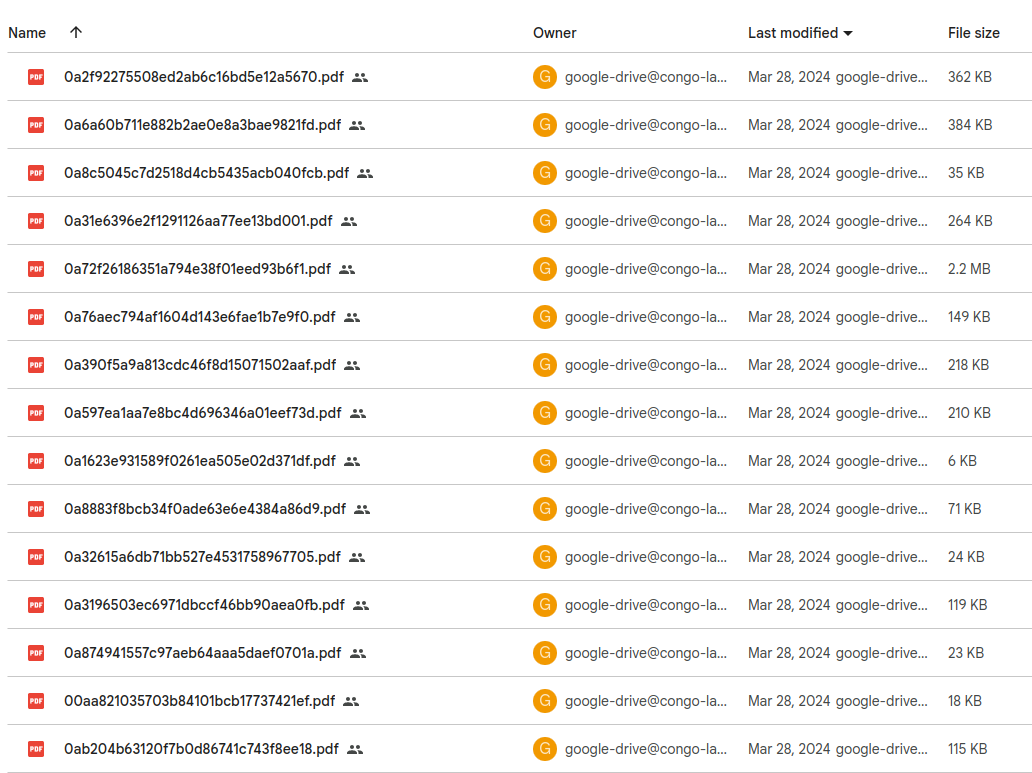
\includegraphics[width=15cm]{gfx/fig-google-drive.png}
    \caption{Documents sur Google Drive après téléchargement}
    \label{fig:crawler-architecture}
\end{figure}

\paragraph{Implémentation Récursive} \hspace{0pt}

Avec l'ajout d'une implémentation récursive à notre arsenal, notre crawler transcende les limitations précédentes et s'aventure désormais au-delà d'une page unique. Cette version avancée de notre crawler dispose désormais de la capacité de naviguer méthodiquement à travers un site entier, identifiant et téléchargeant non seulement les documents disponibles sur l'\ac{url} de départ mais aussi en suivant les liens vers d'autres pages pour récupérer les fichiers \ac{pdf} associés.

\begin{listing}[!ht]
\begin{minted}{python}
from urllib.parse import urljoin, urlparse, urlunparse
from urllib.request import urlretrieve

def remove_fragment(url):
        parsed_url = urlparse(url)
        clean_parsed_url = parsed_url._replace(fragment="")
        return urlunparse(clean_parsed_url)
\end{minted}
\caption{Fonction de nettoyage d'\ac{url}}
\label{appendix:code:python:remove-fragment}
\end{listing}

Le processus débute avec la fonction $remove\_fragment$, qui purifie l'\ac{url} de toute portion inutile, permettant ainsi de concentrer le crawl sur les contenus essentiels des pages. Puis, $recursive\_crawl$ prend le relais, visitant chaque \ac{url} unique seulement une fois grâce à l'ensemble $visited\_urls$ qui assure une trace des pages déjà explorées et prévient les boucles infinies.

Lorsqu'une page est visitée, toute \ac{url} se terminant par $.pdf$ est immédiatement transmise à $download_pdf$, qui procède au téléchargement du fichier et le sauvegarde dans un emplacement spécifique sur Google Drive. Tous les autres liens sont examinés et suivis s'ils appartiennent au même domaine que l'\ac{url} de départ, et ce processus se poursuit de façon récursive. C'est une exploration en profondeur, déployant une toile d'araignée qui s'étend sur l'intégralité du site.

\begin{listing}[!ht]
\begin{minted}{python}
def recursive_crawl(start_url, url, visited_urls):
        url = remove_fragment(url)
        if url in visited_urls:
            return

        visited_urls.add(url)
        print(url)

        try:
            response = requests.get(url)
            response.raise_for_status()
            soup = BeautifulSoup(response.text, 'html.parser')

            if url.lower().endswith('.pdf'):
                download_pdf(url, '/content/drive/MyDrive/DATA/LawLLM/PDF/')
                print(f"File-Downloaded: {url}")

            for link in soup.find_all('a', href=True):
                href = link['href']

                if not urlparse(href).scheme:
                    next_url = urljoin(url, href)
                    recursive_crawl(start_url, next_url, visited_urls)

                elif urlparse(href).hostname == urlparse(start_url).hostname:
                    recursive_crawl(start_url, href, visited_urls)

        except Exception as e:
            print(f"Error while processing {url}: {e}")

def recursive_crawl_link(start_url, destination):
    visited_urls = set()
    recursive_crawl(start_url, start_url, visited_urls)
\end{minted}
\caption{Implémentation récursive du crawler}
\label{appendix:code:python:remove-fragment}
\end{listing}

Cela transforme notre crawler en un outil dynamique et exhaustif, capable d'extraire méthodiquement une richesse d'informations et de ressources souvent enfouies dans la structure des sites web. En exploitant $recursive\_crawl$, nous pouvons cartographier un domaine entier, saisissant non seulement la superficie mais aussi plongeant dans les couches les plus profondes de contenu.

L'implémentation récursive signifie également que notre crawler peut fonctionner avec une autonomie et une efficacité élevées, nécessitant une supervision minimale et permettant aux chercheurs et aux professionnels de se concentrer sur l'analyse et l'exploitation des données collectées plutôt que sur le processus de collecte lui-même.

Cette méthode enrichit considérablement notre ensemble de données, non seulement en volume mais aussi en variété, fournissant une image complète et nuancée du domaine juridique congolais, qui est notre objectif premier. Elle souligne l'efficacité de la programmation récursive dans des applications pratiques telles que le web scraping, démontrant comment une approche algorithmique bien pensée peut considérablement simplifier des tâches autrement ardues et complexes.

\begin{figure}[H]
    \centering
    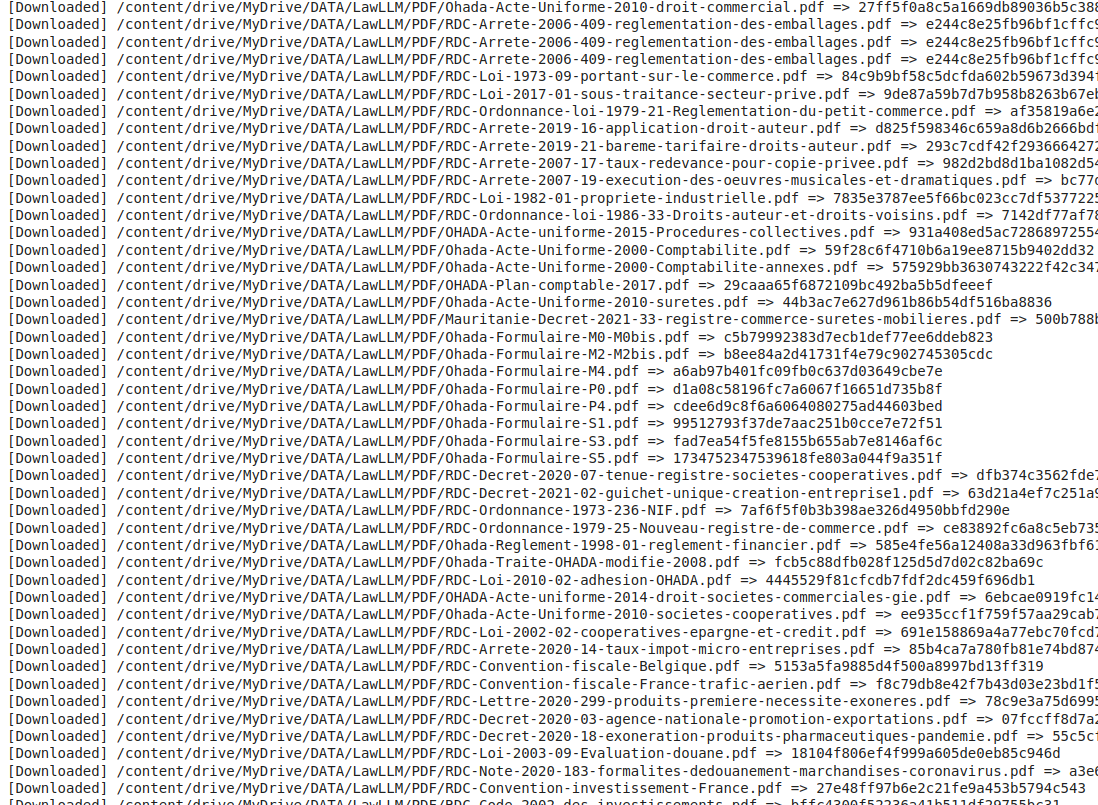
\includegraphics[width=15cm]{gfx/fig-crawler-downloading.png}
    \caption{Téléchargement en cours, approche itérative}
    \label{fig:crawler-downloading}
\end{figure}

\begin{figure}[H]
    \centering
    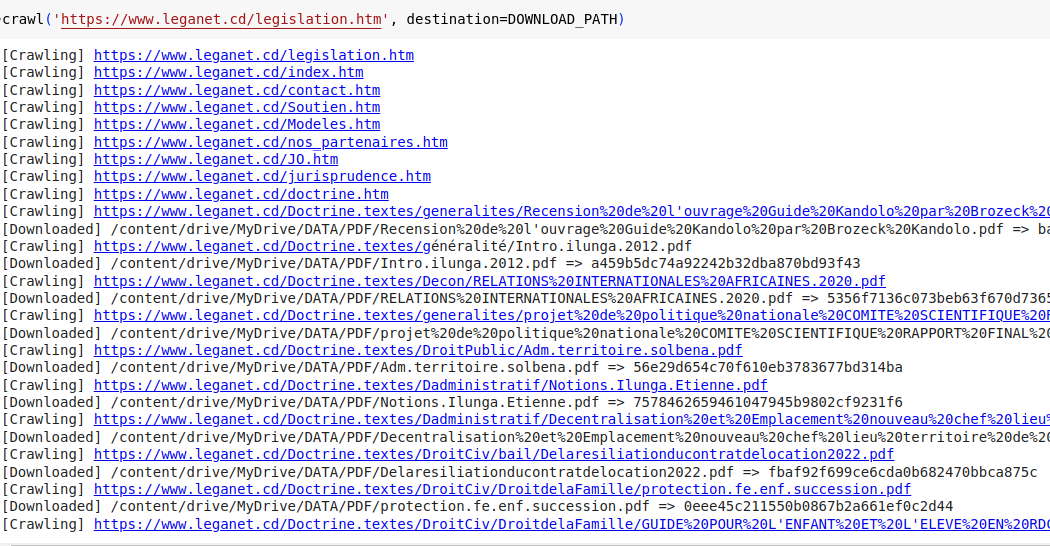
\includegraphics[width=15cm]{gfx/fig-download-recursive.png}
    \caption{Téléchargement en cours, approche récursive}
    \label{fig:crawler-downloading}
\end{figure}

\subsection{Pré-traitement et Formalisations des données}

Après avoir mené à bien le téléchargement de plus de 4000 documents, il est essentiel de reconnaître que bien que ces fichiers soient une mine d'informations, leur forme brute n'est pas directement utilisable. Par conséquent, l'étape de pré-traitement devient cruciale. Dans notre contexte, le pré-traitement consiste principalement à convertir le contenu de ces documents \acs{pdf} en texte exploitable.

Le processus d'extraction de texte des PDF est un défi en soi, car il implique de décoder les diverses manières dont le contenu est encapsulé dans un document \acs{pdf}. Cela peut inclure la gestion de la mise en page complexe, l'extraction de texte à partir d'images incorporées par \ac{ocr} et la préservation de la structure sémantique des informations.

\paragraph{Extraction du texte} \hspace{0pt}

L'extraction de texte à partir de documents PDF est une opération qui peut être réalisée avec efficacité en utilisant la bibliothèque Fitz, également connue sous le nom de PyMuPDF \footnote{\href{https://pymupdf.readthedocs.io/en/latest/}{https://pymupdf.readthedocs.io/en/latest/}}.

\paragraph{Extraction du texte sur image} \hspace{0pt}

Pour extraire du texte à partir d'images, telles que des documents scannés ou numérisés, nous faisons appel à Tesseract. Tesseract est un moteur d'\ac{ocr} open source, considéré comme l'un des plus précis disponibles. L'\ac{ocr} est une technologie qui permet de convertir différents types de documents, tels que des images numérisées de texte imprimé, des captures d'écran ou des images contenant du texte, en données de texte modifiables et recherchables \cite{smith_tesseract_2007}.


\begin{listing}[!ht]
\begin{minted}{python}
def extract_text(pdf_path):
    doc = fitz.open(pdf_path)
    text_content = []

    for page_num in range(len(doc)):
        page = doc.load_page(page_num)
        text = page.get_text("text")
        text_content.append({
            'page': page_num + 1, 
            'type': 'text', 
            'content': text
        })

        # Extract images and use OCR if necessary
        image_list = page.get_images(full=True)
        for image_index, img in enumerate(page.get_images(full=True)):
            # Get the XREF of the image
            xref = img[0]
            # Extract the image bytes
            base_image = doc.extract_image(xref)
            image_bytes = base_image["image"]
        
            # Open the image with PIL
            image = Image.open(io.BytesIO(image_bytes))
            ocr_text = pytesseract.image_to_string(
                image, 
                lang='eng',
                output_type=Output.STRING
            )
            
            extracted_content.append({
                'page': page_num + 1, 
                'type': 'image', 
                'content': ocr_text, 
                'image_index': image_index + 1
            })

    doc.close()
    return text_content
\end{minted}
\caption{Extraction du contenu d'un document PDF}
\label{appendix:code:python:remove-fragment}
\end{listing}


\newpage
\newpage
\subsection{Pré-traitement et Formalisations des données}
\subsection{Stockage des données}

\section{Adaption du LLM avec l'approche RAG}
\subsection{Pré-traitement et Création des Embeddings}
\subsection{Construction de l'index de recherche}
\subsection{Fonction de distance vectorielle}
\subsection{Requêtes sur l'index de recherche}
\subsection{Déploiement de l'index de recherche}

\section{Adaption du LLM avec l'approche Fine-tuning}
\subsection{Pré-traitement et Formalisation}
\subsection{Création du modèle}
\subsection{Déploiement du modèle}

\section{Conception de l'application Web}
\subsection{Modélisation de la base de données}
\subsection{Architecture et choix technologique}
\subsection{Diagrammes UML}
\subsection{Développement}

\section{Déploiement et mis en production}
